\section{Results}\label{sec:results}
All numbers come from one end-to-end run of \code{scripts/selftest.sh} on a freshly created cluster (empty volumes). The host was an Apple-silicon MacBook (10 CPUs) running Docker Desktop with 8\,GB of memory. All 13 containers share this one machine, so absolute latencies are not representative of a real deployment. The \emph{differences} between settings and the \emph{timing} of failure handling are the meaningful results.

\begin{table*}[t]
\caption{HBase compared with Cassandra and MongoDB}\label{tab:compare}
\small
\begin{tabularx}{\textwidth}{@{}lXXX@{}}
\toprule
 & Apache HBase & Apache Cassandra & MongoDB (replica set / sharded) \\
\midrule
Partitioning & key ranges (regions), split on size & consistent hashing with virtual nodes & ranged or hashed chunks per shard \\
Writers per key & 1 (region primary) & any replica (leaderless) & 1 (shard primary) \\
Replication & below the database, in HDFS (3 copies of WAL and HFiles) & between database nodes, $N$ replicas & oplog shipped from primary to secondaries \\
Consensus & ZooKeeper (Zab) for membership and master; leases for regions & none for normal writes; Paxos for lightweight transactions & Raft-like election among data replicas \\
Default consistency & strong per row & tunable ($R{+}W{>}N$ with QUORUM) & primary reads, majority write concern \\
Conflict handling & none needed (single writer); timestamp per cell & last-write-wins, read repair, hinted handoff, Merkle trees & none needed; rollback of unreplicated writes after failover \\
Partition behaviour & CP: minority regions unavailable & AP at ONE, CP at QUORUM & CP: minority side has no primary \\
\bottomrule
\end{tabularx}
\end{table*}

\subsection{Baseline: durability and consistency settings}
Table~\ref{tab:bench} shows 2000 sequential operations per setting from one client, after a warm-up of 500 writes. Every request crosses the Python client, the Thrift gateway and the RegionServer, which costs about 0.4\,ms in total.

\begin{table}[t]
\caption{Latency and throughput per setting (one client, 2000 ops each)}\label{tab:bench}
\small
\begin{tabularx}{\columnwidth}{@{}Xrrrr@{}}
\toprule
Setting & ops/s & p50 ms & p95 ms & p99 ms \\
\midrule
Write \code{SKIP\_WAL}  & 1830 & 0.51 & 0.81 & 1.42 \\
Write \code{ASYNC\_WAL} & 2016 & 0.40 & 0.91 & 2.91 \\
Write \code{SYNC\_WAL}  & 1051 & 0.78 & 1.62 & 4.07 \\
\midrule
Read \code{STRONG}      & 1706 & 0.47 & 0.98 & 2.17 \\
Read \code{TIMELINE}    & 2261 & 0.40 & 0.65 & 0.97 \\
\bottomrule
\end{tabularx}
\end{table}

\textbf{Durability.} \code{SYNC\_WAL}, the default, halves throughput compared with the two asynchronous modes and adds about 0.3--0.4\,ms to the median and 1--3\,ms to the tail. This is the cost of waiting for the three-DataNode pipeline before acknowledging. \code{SKIP\_WAL} and \code{ASYNC\_WAL} are within measurement noise of each other, because neither waits for HDFS. What separates them is the failure behaviour shown in Sec.~VII-E, not their speed.

\textbf{Read consistency.} In a healthy cluster the primary always answers within the 10\,ms \code{primaryCallTimeout}, so all 2000 \code{TIMELINE} reads were served by the primary, and \emph{none} was stale. Both modes therefore take the same path, and the remaining gap is a warm-cache and ordering effect, not a property of the mode. Timeline consistency changes nothing while the system is healthy. It only matters during failures (Sec.~VII-B).

\textbf{Freshness of secondaries.} To isolate replication lag, we wrote a new value and immediately read it from secondary replica~1 (\code{targetReplicaId=1}). In all 100 probes the first read returned the old value, so the secondary was always behind. The new value appeared after a median of 2.0\,s (p95 4.9\,s, maximum 5.0\,s). Secondaries are updated by an asynchronous replication peer that tails the primary's WAL in batches. Their lag is therefore of the order of seconds, not milliseconds, which is why timeline reads must be treated as possibly stale.

A first attempt revealed a further detail. Before the primary had flushed even once, secondary replicas did not serve reads at all. HBase makes a secondary wait for a flush marker from the primary before it opens for reads (\code{hbase.region.replica.wait.for.primary.flush}). Our table-creation job therefore flushes the new table once.

\subsection{RegionServer crash}\label{sec:rscrash}
We killed \code{rs3}, which held the primaries of 3 of the 8 regions and did not host \code{hbase:meta}, with \code{docker kill}. Client traffic was running at 40 writes/s (Fig.~\ref{fig:rscrash}). Observed sequence:
\begin{itemize}
\item $t{=}20$\,s: crash. Within one second the three affected regions stopped answering. Workers writing to them blocked until the 4\,s client operation timeout and then reported failures. The other five regions continued at full rate, so total write throughput dropped from 40 to 25 ops/s and never to zero.
\item $t{=}21$--36\,s: \textbf{16 s of write unavailability} for the affected regions. This matches the 10\,s ZooKeeper session timeout plus about 5\,s for the master's \code{ServerCrashProcedure}: splitting the WAL, reassigning the regions and replaying the edits.
\item During this window, 12 \code{STRONG} reads failed. The \code{TIMELINE} reads of the same rows all succeeded, 13 of them with the stale flag set because a secondary answered.
\item $t{=}37$\,s: all eight regions were writable again on the two surviving servers. At $t{=}65$\,s \code{rs3} was restarted and rejoined with no regions, until the balancer moved some back.
\end{itemize}
\code{verify.py} re-read all 3750 acknowledged writes, and \textbf{none was lost}. The 15 failed writes were not present either, so each client-side timeout corresponded to a write that had not been applied.

\begin{figure*}[t]
\centering
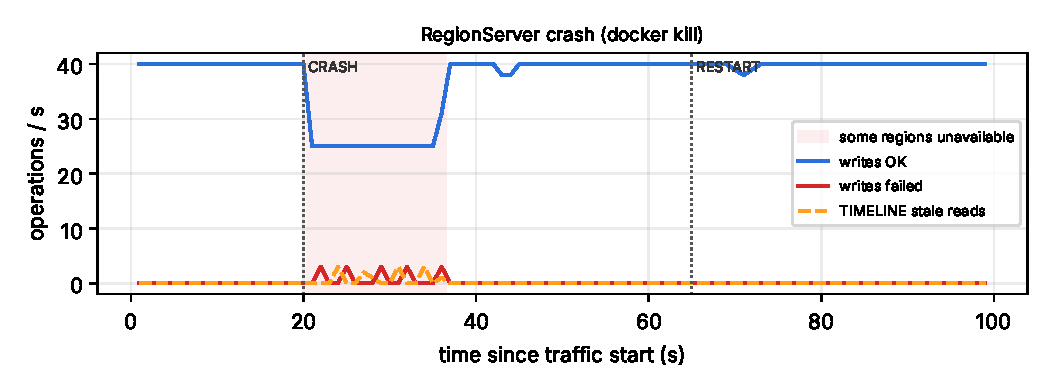
\includegraphics[width=0.8\textwidth]{fig/rs_crash.pdf}
\caption{RegionServer crash under load. The shaded area marks seconds in which at least one region was unavailable. Only the regions of the crashed server stop, and timeline reads stay available with stale results.}\label{fig:rscrash}
\end{figure*}

\subsection{Network partition}
We disconnected \code{rs1}, which held 4 primaries, from the Docker network for 50\,s (Fig.~\ref{fig:partition}). From the cluster's point of view this looks like a crash, and the timing was identical: \textbf{16 s} of unavailability for the four affected regions ($t{=}21$--36\,s), followed by reassignment. The isolated server could not reach ZooKeeper, the HMaster or the DataNodes. When the network was restored at $t{=}71$\,s, its ZooKeeper session had already expired and its WAL leases had been recovered by the master. The server therefore shut itself down instead of serving its old regions again, and the script restarted it as a new incarnation. No client ever saw two servers accept writes for the same region. Of 4463 acknowledged writes, \textbf{0 were lost}. 8 writes and 8 \code{STRONG} reads failed during the window, while \textbf{0 \code{TIMELINE} reads failed}. This run demonstrates the CP choice directly: the minority side loses availability, and the majority side stays consistent.

\begin{figure*}[t]
\centering
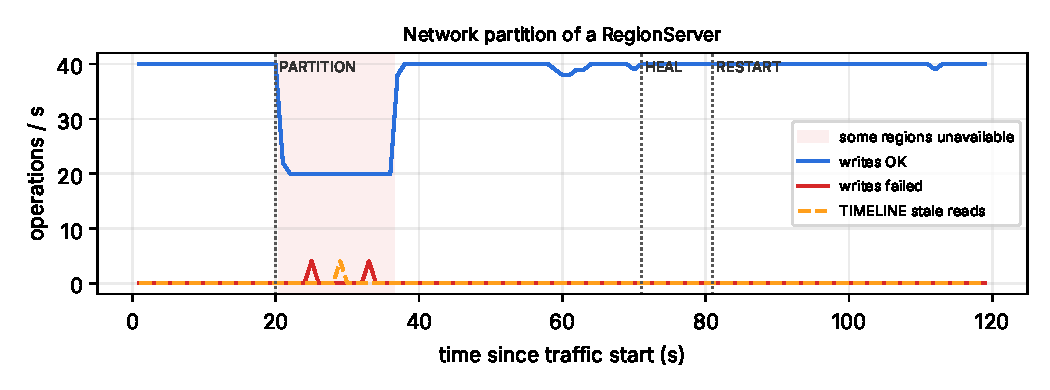
\includegraphics[width=0.8\textwidth]{fig/partition.pdf}
\caption{Network partition of one RegionServer. The isolated server is fenced and later restarts as a new instance. The data path recovers on the majority side after about 16\,s.}\label{fig:partition}
\end{figure*}

\subsection{Master failover and ZooKeeper leader failure}
Fig.~\ref{fig:control} shows both runs. \textbf{HMaster.} Killing the active \code{hmaster1} had \textbf{no effect on client traffic}: 2392 writes, 0 failures. Masters are not on the data path. Within the 26\,s observation window the backup \code{hmaster2} had acquired the \code{/hbase/master} lock and become active. The restarted \code{hmaster1} rejoined as backup.

\textbf{ZooKeeper.} Killing the ZooKeeper leader \code{zk3} triggered a Zab election, and five seconds later \code{zk2} was the new leader, with \code{zk1} as follower and \code{zk3} down. Traffic again saw \textbf{0 failures} out of 1792 writes. The two surviving servers still formed a quorum, and the clients' sessions moved to them before the 10\,s timeout. The restarted \code{zk3} rejoined as follower.

\begin{figure}[t]
\centering
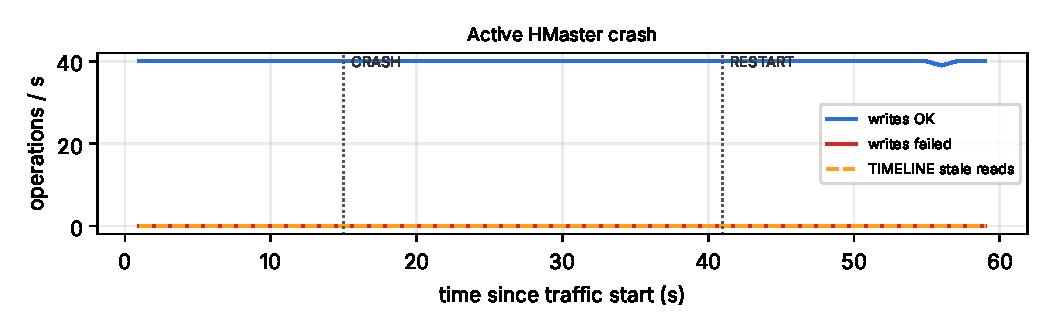
\includegraphics[width=\columnwidth]{fig/master.pdf}\\[2pt]
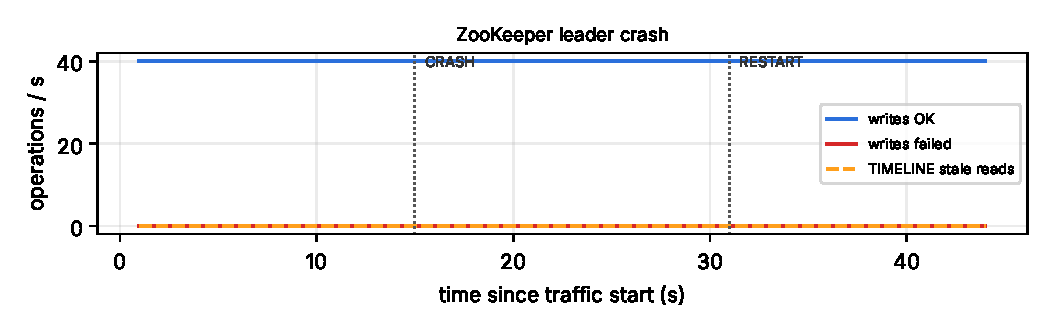
\includegraphics[width=\columnwidth]{fig/zk.pdf}
\caption{Control-plane failures: the active HMaster (top) and the ZooKeeper leader (bottom). Write throughput stays at 40 ops/s with no failures.}\label{fig:control}
\end{figure}

\subsection{What the WAL buys: crash with unflushed data}\label{sec:walloss}
We wrote 400 rows with \code{SKIP\_WAL} and 400 with \code{SYNC\_WAL}, spread over all regions, verified that all 800 were readable, and then killed \code{rs2} before any flush. Table~\ref{tab:walloss} shows the state after recovery. Every \code{SKIP\_WAL} row whose region was hosted on \code{rs2}, 50 rows in each of its 4 regions, disappeared. Those rows had existed only in that server's MemStore. Every \code{SYNC\_WAL} row survived, because the WAL on HDFS was split and replayed on the new servers. The durability setting is therefore a \emph{correctness} decision, not a performance tweak: \code{SKIP\_WAL} gained nothing measurable over \code{ASYNC\_WAL} in Table~\ref{tab:bench}, but loses every unflushed row on a crash.

\begin{table}[t]
\caption{Rows readable after a RegionServer crash before any flush}\label{tab:walloss}
\small
\begin{tabularx}{\columnwidth}{@{}Xrrr@{}}
\toprule
Durability & written & after recovery & lost \\
\midrule
\code{SKIP\_WAL} & 400 & 200 & 200 (4 regions $\times$ 50) \\
\code{SYNC\_WAL} & 400 & 400 & 0 \\
\bottomrule
\end{tabularx}
\end{table}

\subsection{Summary of fault experiments}
\begin{table}[t]
\caption{Fault experiments under live traffic (40 writes/s)}\label{tab:chaos}
\small
\begin{tabularx}{\columnwidth}{@{}Xrrrr@{}}
\toprule
Fault & unavail. & acked & failed & lost \\
\midrule
RegionServer crash (3/8 regions) & 16 s & 3750 & 15 & 0 \\
RegionServer partition (4/8) & 16 s & 4463 & 8 & 0 \\
Active HMaster crash & 0 s & 2392 & 0 & 0 \\
ZooKeeper leader crash & 0 s & 1792 & 0 & 0 \\
\bottomrule
\end{tabularx}
\footnotesize Unavailability applies only to the regions of the failed server. Other regions were unaffected. \code{TIMELINE} reads never failed in any experiment.
\end{table}

Table~\ref{tab:chaos} summarizes the four experiments. The results line up with the analysis in Sections~\ref{sec:cons}--\ref{sec:ft}:
\begin{enumerate}
\item failure detection is bounded by the ZooKeeper session timeout;
\item unavailability is limited to the regions of the failed server;
\item control-plane failures (master, ZooKeeper leader) do not interrupt the data path;
\item fencing prevents a partitioned server from coming back with stale ownership;
\item no acknowledged write is lost as long as the WAL is used.
\end{enumerate}

\section{Discussion}
\textbf{Tuning the detection window.} About two thirds of the 16\,s outage is the session timeout. We chose 10\,s, down from the 90\,s default. In production a lower value is risky: a garbage-collection pause longer than the timeout makes a healthy server look dead. Fencing keeps this safe, but it is expensive, because the server aborts and all its regions move. Operators therefore trade mean time to recovery against false suspicion. This is the same trade-off as the election timeout in Raft.

\textbf{When timeline reads are worth it.} Region replicas triple the memory used for MemStores and block caches, and they add replication traffic. In exchange, reads stay available through the outage window shown in Fig.~\ref{fig:rscrash}. They suit read-mostly workloads that tolerate seconds of staleness, such as product catalogs or dashboards. They do not suit read-modify-write logic, for which \code{STRONG} reads or \code{checkAndMutate} are required.

\textbf{Comparison with other systems.} Table~\ref{tab:compare} places HBase next to the two systems most often compared with it. Cassandra's leaderless design can stay writable on both sides of a partition and therefore needs the anti-entropy machinery that HBase does not have. MongoDB, like HBase, has one writer per shard, but it elects that writer with a Raft-like protocol among the data replicas themselves. HBase delegates election to ZooKeeper and durability to HDFS.



\textbf{Lessons from building the cluster.} Three problems we hit while building the environment taught us more about HBase than the documentation did:
\begin{itemize}
\item \emph{Identity matters.} RegionServers first aborted with ``Master passed us a different hostname''. The master had reverse-resolved a container's IP to \code{rs1.hw3net}, while the server called itself \code{rs1}. HBase treats a server's name, port and startcode as its identity, because that identity is what fencing and the dead-server list are keyed on. A mismatch is therefore fatal by design.
\item \emph{Secondaries are not readable on day one.} Timeline reads to a new table failed until the primary had flushed once, because a secondary waits for a flush marker before it trusts its own view.
\item \emph{Dead servers are remembered.} After the failed first starts, the master listed the aborted incarnations as dead servers until their crash procedures finished. Our start-up check had to accept ``3 servers, $n$ dead'' instead of requiring 0 dead.
\end{itemize}

\textbf{Limits of our setup.} All containers share one host and one disk, so the HDFS ``replicas'' are not independent failure domains, and absolute latencies are dominated by the Thrift hop. A partition created with \code{docker network disconnect} is symmetric and clean. Real partitions can be asymmetric or flapping, which would exercise the same fencing paths in more complex orders. We did not test DataNode failures under load, losing a ZooKeeper quorum (2 of 3 servers), or crashing the server that hosts \code{hbase:meta}. In the last case, location lookups for \emph{all} regions would wait until meta is reassigned.
